\chapter{$e/ m$ of The Electron}
\section{General Discussion}
The ``discovery'' of the electron by J. J. Thomson in 1897 refers to the experiment in which it was shown that ``cathode rays'' behave as beams of particles, all of which have the same ratio of charge to mass, $e/m$. Since that time, a number of experiments have been devised using electric and magnetic fields to precisely measure $e/m$ for the electron. When combined with the value of the electron's charge, which is measured in the Millikan Oil Drop Experiment, the determination of $e/m$ leads to an accurate value of the mass of the electron.\myskip

In the present experiment, electrons are emitted at a very low velocity from a heated filament, then accelerated through an electrical potential $V$ to a final velocity $v$, and finally bent in a circular path of radius $r$ in a magnetic field $B$. The entire process takes place in a sealed glass tube in which the path of the electrons can be directly observed. During its manufacture, the tube was evacuated, and a small amount of mercury was introduced before the tube was sealed off. As a result, there is mercury vapor in the tube. When electrons in the beam have sufficiently high kinetic energy ($10.4\,\mathrm{eV}$ or more), a small fraction of them will collide with and ionize mercury atoms in the vapor. Recombination of the mercury ions, accompanied by the emission of characteristic blue light, then occurs very near the point where the ionization took place. As a result, the path of the electron beam is visible to the naked eye. \myskip

The tube is set up so that the beam of electrons travels perpendicular to a uniform magnetic field $B$. $B$ is proportional to the current $I$ through a pair of large diameter coils (so-called ``Helmholtz Coils'') in which the coil separation is selected to produce optimum field uniformity near the center.

\section{Experimental Apparatus}
\subsection{The Sealed Glass Tube}
\begin{figure}[h]
\centering
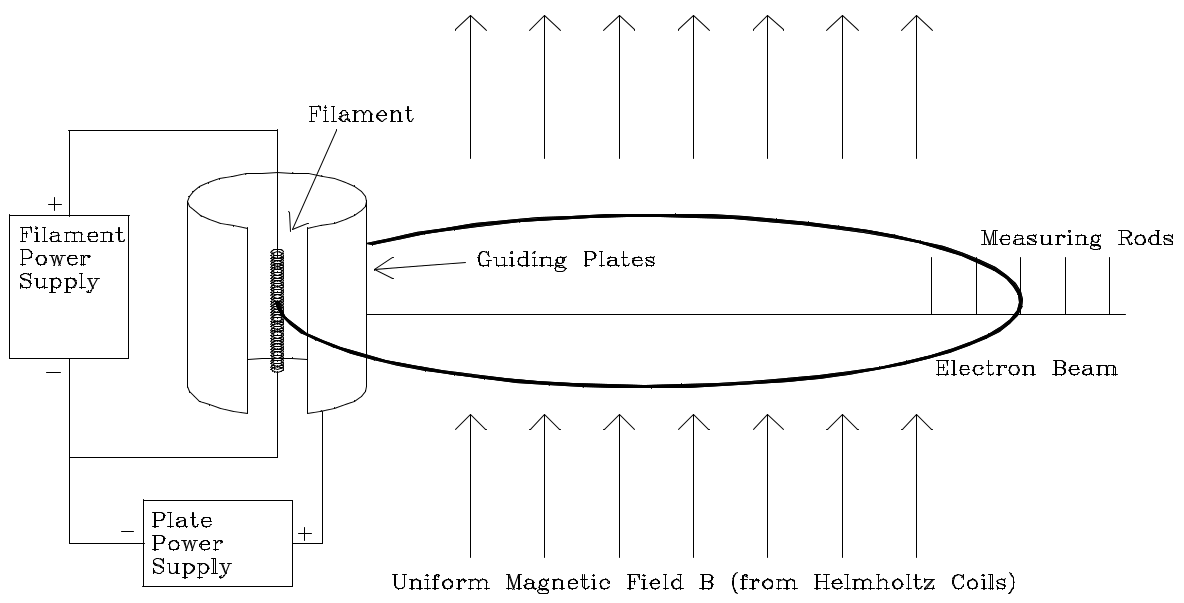
\includegraphics[width=0.8\textwidth]{./Exp6/pic/image1.png}
\caption{Diagram of the Interior of the Sealed Glass Tube}
\label{fig:tube}
\end{figure}

Figure {\ref{fig:tube}} shows the filament surrounded by a small cylindrical plate. The filament is heated by passing a current directly through it. A variable positive potential difference of up to 100 volts is applied between the plate and the filament in order to accelerate the electrons emitted from the filament. Some of the accelerated electrons come out as a narrow beam through a slit in the side of the cylinder. The entire tube is located inside a set of coils, which produce a uniform magnetic field $B$ perpendicular to the electron beam. The magnitude of the field can be adjusted until the resultant circular path of the electron beam just reaches one of the measuring rods. These rods are located along a cross bar, which extends from the cylinder in a direction perpendicular to that in which the electron beam was emitted--i.e., along a diameter of the circular orbits.

\subsection{The Helmholtz Coils and Uniform Magnetic Field}
The magnetic field produced at the position of the electron beam by a current $I$ flowing through the coils must be computed. For a single turn of wire of radius $R$, the field on the axis at a distance $x$ from the plane of the loop is given by:
\begin{equation}
  B'=\frac{\mu_{0}R^{2}I}{2(R^2+x^2)^{3/2}}.
\end{equation}

For the arrangement in Figure {\ref{fig:coils}}, there are two loops with $N$ turns each, separated by a distance equal to the coil radius $R$. The coils contribute equally to the field at the center:
\begin{equation}
  B_{I}=\frac{\mu_{0}R^2NI}{\big[R^2+(R/2)^2\big]^{3/2}}=\frac{4\pi\times 10^{-7}NI}{R(1+\frac{1}{4})^{3/2}}=\mathrm{constant}\times I\, \mathrm{Tesla}
\label{eq:bi}
\end{equation}
where $N = 72$ is the number of turns of each coil and $R = 33\, \mathrm{cm}$ is the radius of the coils used.\myskip
\begin{figure}[h]
\centering
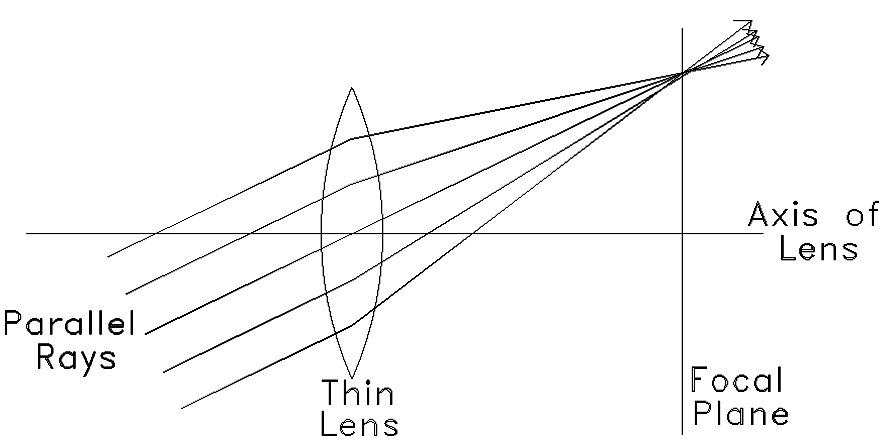
\includegraphics[width=0.8\textwidth]{./Exp6/pic/image2.png}
\caption{Helmholtz coils used to produce a uniform magnetic field.}
\label{fig:coils}
\end{figure}

This arrangement, called a pair of \textbf{Helmholtz coils}, yields a remarkably uniform field in the region at the center.\myskip

The net field $B$ in which the electrons move is not $B_I$ alone, however. We also feel some of the Earth's own magnetic field, $B_E$. If the equipment is oriented such that these two fields, $B_I$ and $B_E$ are parallel, then the net field will be the sum of the two parts. And if $B_I$ is set to be in the opposite direction to $B_E$, then the we have
\begin{equation}
  B=B_{I}-B_{e}.
\label{eq:b}
\end{equation}

\subsection{The Trajectories of the Electrons in the Glass Tube}
If an electron of charge $e$ and mass $m$ starts nearly from rest and is accelerated through a potential difference $V$ to a final velocity $v$, then
\begin{equation}
  \frac{1}{2}mv^2=eV\quad \mathrm{or}\quad \frac{e}{m}=\frac{v^2}{2V}
\label{eq:ev}
\end{equation}

If the electron then enters a uniform magnetic field $B$ which is perpendicular to its velocity, it will move in a circular orbit of radius $r$, where
\begin{equation}
  \frac{mv^2}{r}=evB\quad\mathrm{or}\quad \frac{e}{m}=\frac{v}{Br}
\label{eq:eb}
\end{equation}

If it were possible to measure the velocity directly, then $e/m$ could be determined by measurements of either the electric or magnetic field alone. Since a direct measurement of $v$ is not feasible in this experiment, $e/m$ can best be determined from the combination of electric and magnetic fields used. Specifically, by eliminating $v$ from equations ({\ref{eq:ev}}) and ({\ref{eq:eb}}), $e/m$ can be expressed directly in terms of $V$, $B$, and $r$.\myskip

Instead of determining $e/m$ from a single measurement of $r$ for given values of $V$ and $B$, however, it is preferable to measure the variation of $r$ with $B$ (or $I$) at fixed values of $V$. In particular, the data can be presented in convenient form by plotting the \textbf{curvature} $1/r$ as a linear function of $I$.
\begin{equation}
  \frac{1}{r}=\sqrt{\frac{e}{m}\frac{1}{2V}}B_{I}-\sqrt{\frac{e}{m}\frac{1}{2V}}B_{e}
\label{eq:r}
\end{equation}

Derive ({\ref{eq:r}}) from ({\ref{eq:b}}), ({\ref{eq:ev}}), and ({\ref{eq:eb}}) for your report \underline{before} coming to laboratory.\myskip

Note that equations ({\ref{eq:ev}}), ({\ref{eq:eb}}), and ({\ref{eq:r}}) apply strictly only to electrons with trajectories on the \emph{outside edge} of the beam -- i.e., the most energetic electrons. There are two reasons why some electrons in the beam will have less energy:
\begin{enumerate}
\item There is a small potential difference across the filament caused by the heating current. Only electrons leaving the negative end of the filament are accelerated through the whole potential difference $V$.
\item Some of the electrons in the beam will lose energy through collisions with mercury atoms.
\end{enumerate}

\section{Procedure}
\subsection{Orientation of the Coil and Tube Setup}

For reasons already explained, we would like to orient the Helmholtz coils such that their axes are parallel to the ambient magnetic field.\myskip

\emph{Please exercise extreme care in the following section as you align the Helmholtz coils: the cathode ray tube is very delicate and may break if the coil support is not very firmly secured and falls.  It is recommended that two people handle the coil frame at all times while the coils are being aligned.  Also take care not to touch the dip needle, which is easily bent.}\myskip

In order to align the coils so that their axis is aligned with the ambient magnetic field proceed as follows:
\begin{itemize}
    \item With the coils in the horizontal position, rotate the horizontal arm of the dip needle support so that the needle itself and the plastic protractor are horizontal.  Avoid touching the needle or plastic protractor, and instead turn the arm using the attached lever.
    \item Allow the compass needle to come to a rest.  It is now pointing in the direction of the horizontal component of the ambient field.
    \item Rotate the entire frame by turning the base, until the compass needle is aligned along the $90^\circ$-$270^\circ$ line on the protractor.  The horizontal axis of the cathode ray tube (coaxial with the metal rod) is now aligned with the horizontal component of the ambient field.
    \item Rotate the horizontal arm of the dip needle support so that the needle itself and the plastic protractor are now in a vertical plane.  Avoid touching the needle or plastic protractor, and instead turn the arm using the attached lever.
    \item Allow the needle to come to a rest.  It is now pointing in the direction of the ambient field.
    \item Loosen the wingnut and \textbf{gently} raise one side of the coils.  You want to increase the angle until the dip needle is aligned along the $0^\circ$-$180^\circ$ line on the protractor.  \textbf{Hold the wooden frame rather than the coils as you raise the setup}.
    \item Securely \textbf{tighten the wingnut so that the coils remain in position}.  One person should be supporting the frame while a second person tightens the wingnut.
    \item The coil axis should now be aligned (coaxial) with the ambient magnetic field.
\end{itemize}

\subsection{Preliminary Adjustments}
The supplies and controls for the Helmholtz coils and the filament are permanently wired on a board and are designed to minimize the possibility of damage to the tube or coils. Locate each control, and note the qualitative effects observed when the control is varied. In particular:
\begin{enumerate}[(a)]
\item Figure {\ref{fig:tube}} shows that the filament and its associated lead wires form a small loop. Since a $4\,\mathrm{amp}$ current is required to heat the filament, this loop creates its own measurable magnetic field. The filament coil reversing switch permits you to study the effect of this field. To minimize this effect, rotate the entire tube slightly in its mounting so the electrons come out parallel to the plane of the coils.
\item Note the direction of the coil current for each position of its reversing switch by using the dip needle to check the direction of the resultant field. Knowing the field direction, check the sign of the charge of the particles in the deflected beam. Also, determine whether the earth's field adds to or subtracts from the coil field.
\end{enumerate}

\subsection{Measurement of $e/m$}
With the accelerating voltage at some intermediate value, you may adjust the current in the Helmholtz coils so that the outside edge of the beam strikes the outside edge of each bar in turn.
\begin{itemize}
  \item Measure field current as a function of radius for the highest voltage $V$ which allows you to adjust the beam with respect to all five bars. You can find this voltage by first setting the Helmholtz current to its maximum value and then adjusting the accelerating voltage until electrons pass through the shortest diameter bar.\\ \\

  The tube manufacturer supplies the following values for the \emph{diameters} from the filament to the \emph{outside} of each bar in succession:
  \begin{gather*}
  6.48\,\textrm{cm},\quad 7.75\,\textrm{cm},\quad 9.02\,\textrm{cm},\quad 10.30\,\textrm{cm},\quad 11.54\,\textrm{cm}
  \end{gather*}

  \item For one of your five measurements, test the reproducibility of the current setting as an aid to error analysis. Do this by turning the power supply off and on again. Then readjust the current until the electrons pass through the relevant bar. Do this six times and use the 2/3 method to determine an appropriate uncertainty in field current.

  \item With Microsoft Excel, plot $1/r$ vs. field current $I$ with error bars and draw a best fit line. Calculate the slope of your line and find the error using LINEST.

  \item Using equations ({\ref{eq:r}}) and ({\ref{eq:bi}}), determine $e/m$ from the slope of your best-fit line with error.

  \item Does your calculated $e/m$ value agree with the accepted value within error? The accepted value is $1.758 \times 10^{11}\, \mathrm{coulombs} / \mathrm{kg}$.

  \item Calculate the actual maximum velocity of the electrons in your beam with error found by propagating uncertainties in $e/m$.

  \item Use the intercept of your best-fit line to calculate the strength of the Earth's magnetic field $B_e$ with error.

  \item Discuss the main sources of error in measuring $e\m$ in this experiment.
\end{itemize}
